% ============================================================================
% CSCE 763: Digital Image Processing - Homework 4 Solutions
% ============================================================================

\documentclass[12pt]{article}

% ============================================================================
% PACKAGE IMPORTS
% ============================================================================
\usepackage{amsmath}
\usepackage{graphicx}
\usepackage{amssymb}
\usepackage{tikz}
\usepackage[margin=1in]{geometry}
\usepackage{setspace}
\usepackage{xcolor}
\usepackage{enumitem}
\usepackage{tcolorbox}
\usepackage{fancyhdr}
\usepackage{booktabs}
\usepackage{array}
\usepackage{colortbl}
\usepackage{float}

% ============================================================================
% HEADER AND FOOTER SETUP
% ============================================================================
\pagestyle{fancy}
\setlength{\headheight}{14.5pt}
\fancyhf{}

\fancyhead[L]{Page \thepage}
\fancyhead[C]{CSCE 763}
\fancyhead[R]{JC Vaught}

\renewcommand{\headrulewidth}{0pt}

% ============================================================================
% TIKZ LIBRARIES
% ============================================================================
\usetikzlibrary{shapes.geometric, arrows.meta, positioning, patterns, calc}

% --- USC Brand Colors ---
\definecolor{USC_Garnet}{HTML}{73000A}
\definecolor{USC_Sandstorm}{HTML}{FFF2E3}
\definecolor{USC_Black90}{HTML}{363636}
\definecolor{USC_Black70}{HTML}{5C5C5C}
\definecolor{USC_Black50}{HTML}{A2A2A2}
\definecolor{USC_Black10}{HTML}{ECECEC}
\definecolor{USC_Honeycomb}{HTML}{65780B}
\definecolor{USC_Atlantic}{HTML}{466A9F}
\definecolor{USC_Congaree}{HTML}{1F414D}
\definecolor{USC_Rose}{HTML}{CC2E40}
\definecolor{USC_Grass}{HTML}{CED318}
\definecolor{USC_Horseshoe}{HTML}{65780B}
\definecolor{outputbg}{RGB}{245,245,245}

% ============================================================================
% CUSTOM COLORED BOXES
% ============================================================================
\newtcolorbox{stepbox}[1][Step]{
  colback=white,
  colframe=USC_Garnet,
  fonttitle=\bfseries,
  title={#1},
  sharp corners,
  colbacktitle=USC_Garnet,
  coltitle=white,
}

\newtcolorbox{resultsbox}{
  colback=white,
  colframe=USC_Honeycomb,
  fonttitle=\bfseries,
  title=Results,
  sharp corners,
  colbacktitle=USC_Honeycomb,
  coltitle=white,
}

% ============================================================================
% CUSTOM QUESTION AND PART COMMANDS
% ============================================================================
\newcommand{\question}[1]{%
  \clearpage
  \vspace{0.5cm}
  {\noindent\normalsize \textbf{#1}}
  \vspace{0.2cm}
  \hrule
  \vspace{0.1cm}
  \hrule
  \vspace{0.3cm}
}

\newcommand{\questionpart}[1]{%
  \clearpage
  \vspace{0.5cm}
  {\noindent\normalsize \textbf{#1}}
  \vspace{0.2cm}
  \hrule
  \vspace{0.1cm}
  \hrule
  \vspace{0.3cm}
}

% Graphics path
\graphicspath{{figures/}}

% ============================================================================
% DOCUMENT INFORMATION
% ============================================================================

\title{CSCE 763: Digital Image Processing \\ Homework \#4}
\author{Instructor: Spring 2026 \\ University of South Carolina \\ \textit{Solutions by: JC Vaught}}
\date{Due: 1:15 pm EST, Thursday, Feb 26}

% ============================================================================
% BEGIN DOCUMENT
% ============================================================================

\begin{document}

\maketitle
\setlength{\parindent}{0pt}

\setlist[enumerate,1]{label=\arabic*.}
\setlist[enumerate,2]{label=(\alph*)}

% ============================================================================
% TABLE OF CONTENTS
% ============================================================================

\begin{center}
\begin{tcolorbox}[colback=white, colframe=gray!50!black, colbacktitle=gray!20!white,
                  coltitle=black, sharp corners, boxrule=1pt,
                  title=\Large\bfseries Table of Contents]
\begin{tabular}{p{0.82\textwidth}r}
\textbf{Problem 1: Highboost Filtering (10 pts)} \dotfill & \textbf{\pageref{quest:1}} \\[0.3em]
\textbf{Problem 2: Fourier Transform (20 pts)} \dotfill & \textbf{\pageref{quest:2}} \\[0.3em]
\textbf{Problem 3: Mean/Order-Statistic Filters (30 pts)} \dotfill & \textbf{\pageref{quest:3}} \\[0.3em]
\textbf{Problem 4: Motion Blur Model (20 pts)} \dotfill & \textbf{\pageref{quest:4}} \\[0.3em]
\textbf{Problem 5: Wiener Filter Expression (20 pts)} \dotfill & \textbf{\pageref{quest:5}} \\
\end{tabular}
\vspace{0.2cm}
\end{tcolorbox}
\end{center}

\vspace{0.5cm}

% ============================================================================
% PROBLEM 1: Highboost Filtering
% ============================================================================

\question{Problem 1: Highboost Filtering (10 pts)}\label{quest:1}

As we discussed in class, image sharpening by unsharp masking consists of three steps.
Design a $3 \times 3$ filter for performing highboost filtering with $k=3$ in a single pass through an image,
a single $3 \times 3$ highboost filter performing image sharpening. Assume that the average image is obtained
using the filter shown below:

\[
\frac{1}{9}
\begin{bmatrix}
1 & 1 & 1 \\
1 & 1 & 1 \\
1 & 1 & 1
\end{bmatrix}
\]

\vspace{0.4cm}

\begin{stepbox}[Step 1: Highboost Formula]
Let $f$ be the input image and $\bar{f}=f \otimes h_{\text{avg}}$ be the blurred image. The highboost form is
\[
g = f + k(f-\bar{f}) = (1+k)f - k\bar{f}
\]
For $k=3$:
\[
g = 4f - 3(f\otimes h_{\text{avg}}) = f \otimes \left(4\delta - 3h_{\text{avg}}\right)
\]
So the required single-pass kernel is
\[
h_{\text{HB}} = 4\delta - 3h_{\text{avg}}
\]
\end{stepbox}

\begin{stepbox}[Step 2: Compute the $3\times 3$ Coefficients]
Given
\[
h_{\text{avg}} = \frac{1}{9}
\begin{bmatrix}
1 & 1 & 1 \\
1 & 1 & 1 \\
1 & 1 & 1
\end{bmatrix}
\quad\Rightarrow\quad
3h_{\text{avg}} = \frac{1}{3}
\begin{bmatrix}
1 & 1 & 1 \\
1 & 1 & 1 \\
1 & 1 & 1
\end{bmatrix}
\]
The impulse term $4\delta$ contributes 4 only at the center, 0 elsewhere. Therefore:
\[
h_{\text{HB}} =
\begin{bmatrix}
-\frac13 & -\frac13 & -\frac13 \\
-\frac13 & 4-\frac13 & -\frac13 \\
-\frac13 & -\frac13 & -\frac13
\end{bmatrix}
=
\begin{bmatrix}
-\frac13 & -\frac13 & -\frac13 \\
-\frac13 & \frac{11}{3} & -\frac13 \\
-\frac13 & -\frac13 & -\frac13
\end{bmatrix}
\]
Equivalent scaled form:
\[
h_{\text{HB}} = \frac13
\begin{bmatrix}
-1 & -1 & -1 \\
-1 & 11 & -1 \\
-1 & -1 & -1
\end{bmatrix}
\]
\end{stepbox}

\begin{resultsbox}
The required single-pass $3\times 3$ highboost filter for $k=3$ is
\[
\boxed{
h_{\text{HB}} =
\begin{bmatrix}
-\frac13 & -\frac13 & -\frac13 \\
-\frac13 & \frac{11}{3} & -\frac13 \\
-\frac13 & -\frac13 & -\frac13
\end{bmatrix}
= \frac13
\begin{bmatrix}
-1 & -1 & -1 \\
-1 & 11 & -1 \\
-1 & -1 & -1
\end{bmatrix}}
\]
\end{resultsbox}


% ============================================================================
% PROBLEM 2: Fourier Transform
% ============================================================================

\question{Problem 2: Fourier Transform (20 pts)}\label{quest:2}

Perform Fourier Transform on the function
\[
f(t) =
\begin{cases}
14, & -2w \le t \le 0 \\
3,  & 0 \le t \le 2w \\
0,  & \text{otherwise}
\end{cases}
\]

\vspace{0.4cm}

\begin{stepbox}[Step 1: Use the Continuous FT Definition]
Using the convention
\[
F(u) = \int_{-\infty}^{\infty} f(t)e^{-j2\pi ut}\,dt
\]
we get
\[
F(u)=14\int_{-2w}^{0}e^{-j2\pi ut}\,dt+3\int_{0}^{2w}e^{-j2\pi ut}\,dt
\]
\end{stepbox}

\begin{stepbox}[Step 2: Evaluate the Two Integrals]
For $u\neq 0$:
\[
14\int_{-2w}^{0}e^{-j2\pi ut}\,dt
=\frac{14\left(e^{j4\pi uw}-1\right)}{j2\pi u}
\]
\[
3\int_{0}^{2w}e^{-j2\pi ut}\,dt
=\frac{3\left(1-e^{-j4\pi uw}\right)}{j2\pi u}
\]
Hence
\[
F(u)=\frac{14e^{j4\pi uw}-3e^{-j4\pi uw}-11}{j2\pi u}
\]
\end{stepbox}

\begin{stepbox}[Step 3: Equivalent Trigonometric Form]
Let $\alpha=4\pi uw$. Then
\[
14e^{j\alpha}-3e^{-j\alpha}-11
=11(\cos\alpha-1)+j17\sin\alpha
\]
So
\[
F(u)=\frac{17\sin(4\pi uw)+j11\left[1-\cos(4\pi uw)\right]}{2\pi u},\quad u\neq 0
\]
At $u=0$, from direct area under $f(t)$:
\[
F(0)=\int f(t)dt = 14(2w)+3(2w)=34w
\]
\end{stepbox}

\begin{resultsbox}
\[
\boxed{F(u)=\frac{14e^{j4\pi uw}-3e^{-j4\pi uw}-11}{j2\pi u},\; u\neq0;\qquad F(0)=34w}
\]
Equivalent form:
\[
\boxed{F(u)=\frac{17\sin(4\pi uw)+j11\left[1-\cos(4\pi uw)\right]}{2\pi u},\; u\neq 0}
\]
\end{resultsbox}


% ============================================================================
% PROBLEM 3: Mean/Order-Statistic Filters
% ============================================================================

\question{Problem 3: Mean/Order-Statistic Filters (30 pts)}\label{quest:3}

The white bars in the test pattern shown in Figure 1 are 7 pixels wide and 210 pixels high.
The separation between bars is 17 pixels. What would this image look like after application of a
$9 \times 9$ filter of:

\begin{enumerate}[label=(\alph*)]
\item Arithmetic mean filter
\item Geometric mean filter
\item Harmonic mean filter
\item Contraharmonic mean filter with $Q=1$
\item Contraharmonic mean filter with $Q=0$
\item Contraharmonic mean filter with $Q=-1$
\item Median filter
\item Max filter
\item Min filter
\item Midpoint filter
\end{enumerate}

Hints: you can assume the black background has intensity 0 and white bars have intensity 255.
You can either write a program to implement these filters or represent the image as an array with
numbers and show the results after filtering. You may need to pay attention to the corners of the white bars.

\begin{figure}[H]
\centering
{\color{USC_Garnet}\fbox{\color{black}
\includegraphics[width=0.35\textwidth]{fig1_test_pattern.png}}}
\caption{Figure 1}
\end{figure}

\vspace{0.3cm}

\begin{stepbox}[Step 1: 1D Scan-Line Model]
Analyze one horizontal scan line through bar interiors. Intensities are binary: 255 inside bars and 0 in background.
Bar width $=7$, gap $=17$, period $T=24$. The $9\times 9$ mask has half-width 4 in each direction.
Because $7<9$, no window can be entirely white in the horizontal direction.
\end{stepbox}

\begin{stepbox}[Step 2: Useful Counts for Binary Windows]
For a binary neighborhood containing $n_w$ white pixels and $81-n_w$ black pixels:
\[
\text{arithmetic mean} = \frac{255n_w}{81}
\]
\[
\text{max} = \begin{cases}255,&n_w>0\\0,&n_w=0\end{cases},\qquad
\text{min} = \begin{cases}255,&n_w=81\\0,&n_w<81\end{cases}
\]
\[
\text{midpoint} = \frac{\text{max}+\text{min}}{2}
\]
For bar-interior rows, maximum possible $n_w$ is $7\times 9=63$.
\end{stepbox}

\begin{stepbox}[Filter-by-Filter Outcomes]
\textbf{(a) Arithmetic mean:}
Peak value at bar center is $\frac{63}{81}\cdot255\approx198.3$. Bars become blurred gray ridges; gaps remain dark in the center (since $17-8=9$ columns in each gap never touched by the window).

\textbf{(b) Geometric mean:}
Any zero in window makes the product zero. Every $9\times 9$ window contains at least one zero because bar width is only 7. Output is all black.

\textbf{(c) Harmonic mean:}
Any zero in the window makes denominator infinite, so output is 0. Output is all black.

\textbf{(d) Contraharmonic mean, $Q=1$:}
\[
\hat f = \frac{\sum z^2}{\sum z}
\]
For binary values, if $n_w>0$, this equals 255; if $n_w=0$, equals 0. This is equivalent to a max filter: bars are dilated by 4 pixels on each side (width $7\to15$), still separated because gap becomes 9.

\textbf{(e) Contraharmonic mean, $Q=0$:}
Reduces to arithmetic mean; same result as (a).

\textbf{(f) Contraharmonic mean, $Q=-1$:}
Requires division by $\sum z^{-1}$; zeros cause singular behavior and drive output to 0 whenever any black pixel exists. Since every window contains black pixels, output is effectively all black.

\textbf{(g) Median filter:}
Window size is 81, so median is white iff at least 41 values are white. On interior bar rows, this occurs only where horizontal overlap with the bar is at least 5 columns, which preserves an approximately 7-pixel bar width. Bars remain separated and become cleaner at edges.

\textbf{(h) Max filter:}
Same as (d): binary dilation, width $7\to15$, gap $17\to9$.

\textbf{(i) Min filter:}
Needs all 81 values white. Impossible here because bar width $<9$. Output all black.

\textbf{(j) Midpoint filter:}
Since all-white windows never occur, min is always 0. Where any white is present, max is 255, so midpoint is 127.5. Result is gray dilated bars (value about 128) on black background.
\end{stepbox}

\begin{stepbox}[Computed 9x9 Filter Outputs]
The exact filter outputs computed from the binary $0/255$ test pattern are shown below.
\begin{figure}[H]
\centering
{\color{USC_Garnet}\fbox{\color{black}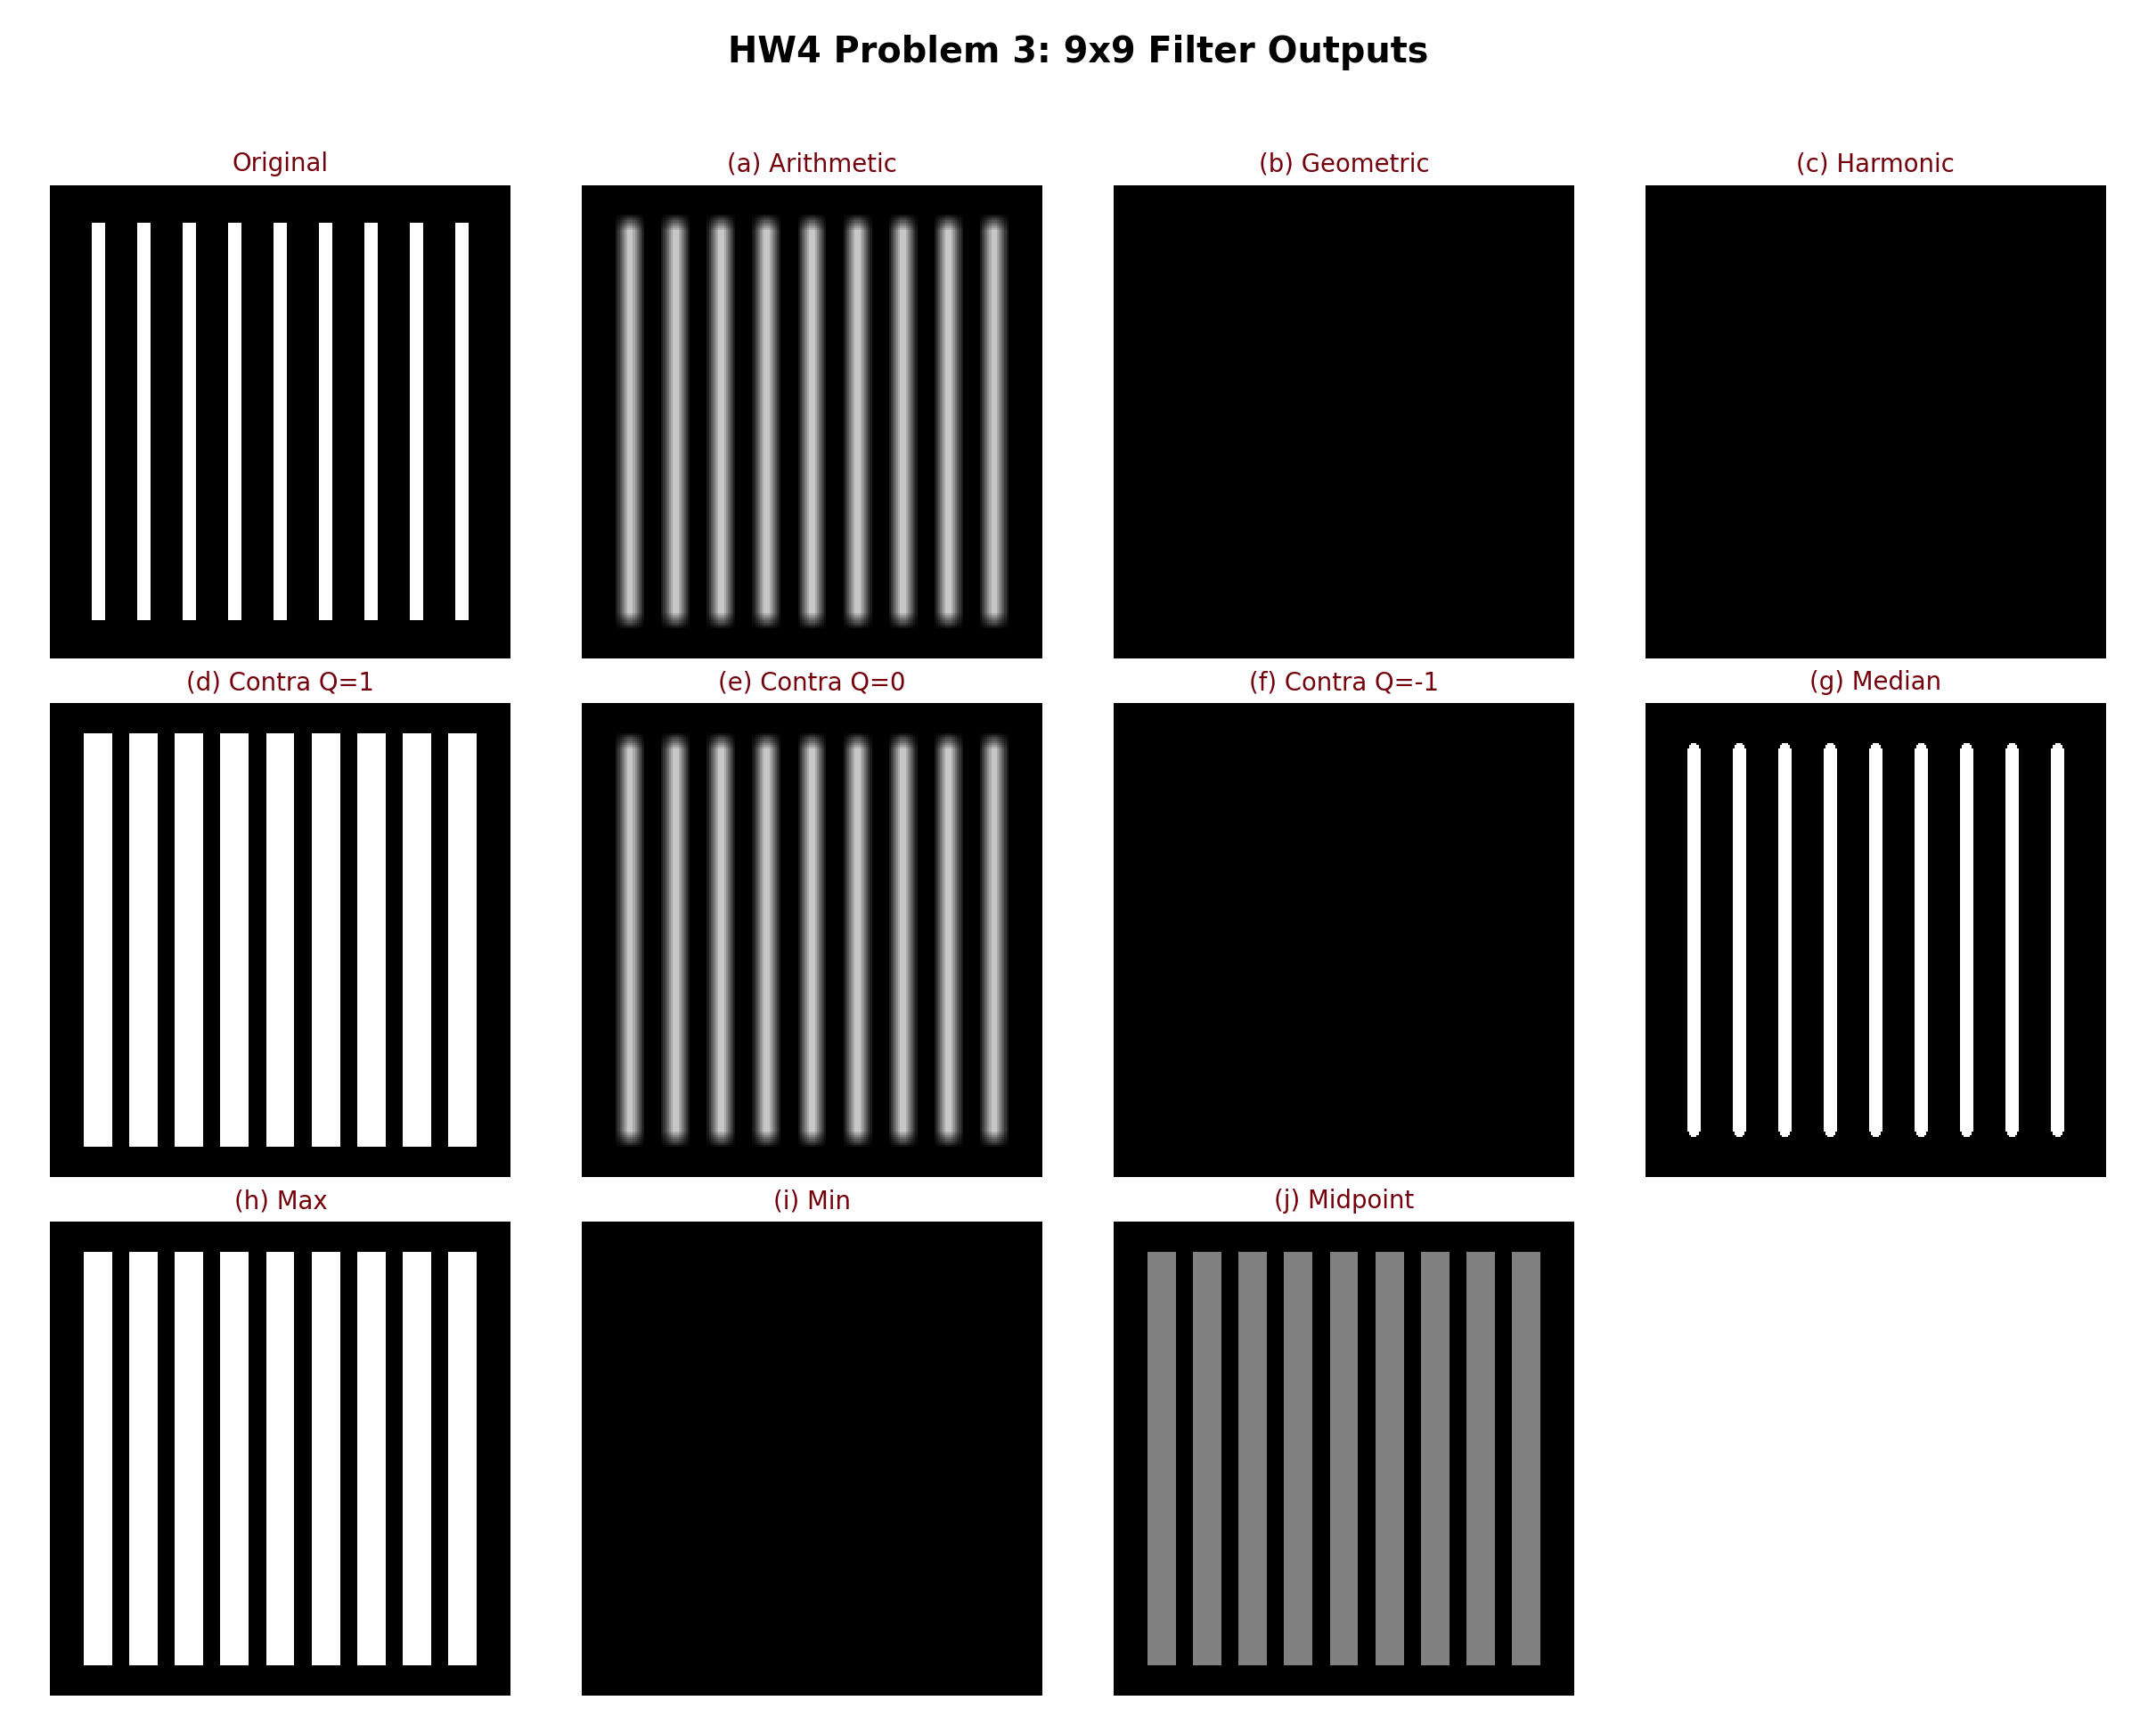
\includegraphics[width=\textwidth]{problem3_filter_outputs/problem3_filter_comparison.png}}}
\caption{Problem 3 computed outputs for filters (a)--(j)}
\end{figure}
\end{stepbox}

\begin{resultsbox}
\begin{center}
\renewcommand{\arraystretch}{1.25}
\begin{tabular}{|>{\centering\arraybackslash}m{0.24\textwidth}|>{\centering\arraybackslash}m{0.68\textwidth}|}
\hline
\textbf{Filter} & \textbf{Result on This Pattern} \\
\hline
Arithmetic mean & Blurred gray bars, peak $\approx198$, bars remain separated. \\
\hline
Geometric mean & All black (0 everywhere). \\
\hline
Harmonic mean & All black (0 everywhere). \\
\hline
Contraharmonic ($Q=1$) & Binary dilation (same as max), width $7\to15$, gap $17\to9$. \\
\hline
Contraharmonic ($Q=0$) & Same as arithmetic mean. \\
\hline
Contraharmonic ($Q=-1$) & Effectively all black due to zeros in every window. \\
\hline
Median & Approx. original bar width preserved; noise-smoothed edges, separation preserved. \\
\hline
Max & Same as $Q=1$: binary dilation. \\
\hline
Min & All black (requires all-255 window, impossible). \\
\hline
Midpoint & Gray dilated bars ($\approx127.5$ where window sees white), black elsewhere. \\
\hline
\end{tabular}
\end{center}
\end{resultsbox}


% ============================================================================
% PROBLEM 4: Motion Blur Model
% ============================================================================

\question{Problem 4: Motion Blur Model (20 pts)}\label{quest:4}

During acquisition, an image undergoes uniform linear motion in the horizontal direction ($y$-direction)
for a time interval $T_1$. The direction of motion then switches to the vertical direction ($x$-direction)
for a time interval $T_2$. Assuming that the time it takes the image to change directions is negligible,
and that shutter opening time and closing time are also negligible, give an expression for the blurring
function, $H(u,v)$.

(Hint: you can refer to the example that the blurring function for motion during acquisition is
\[
H(u,v) = \int_{0}^{T} e^{-j2\pi\left[u\,x_0(t)+v\,y_0(t)\right]}\,dt
\]
)

\vspace{0.4cm}

\begin{stepbox}[Step 1: Piecewise Motion Model]
Let the first segment move along $y$ with constant speed $b$ for $0\le t\le T_1$, and the second segment move along $x$ with constant speed $a$ for $T_1 < t \le T_1+T_2$:
\[
x_0(t)=0,\; y_0(t)=bt, \quad 0\le t\le T_1
\]
\[
x_0(t)=a(t-T_1),\; y_0(t)=bT_1, \quad T_1< t\le T_1+T_2
\]
\end{stepbox}

\begin{stepbox}[Step 2: Split the Integral Over the Two Time Intervals]
\[
H(u,v)=\int_0^{T_1} e^{-j2\pi vbt}\,dt
+\int_{T_1}^{T_1+T_2} e^{-j2\pi\left[u a(t-T_1)+v bT_1\right]}\,dt
\]
\end{stepbox}

\begin{stepbox}[Step 3: Closed Form Expression]
Evaluating each term:
\[
\int_0^{T_1} e^{-j2\pi vbt}\,dt
=\frac{1-e^{-j2\pi vbT_1}}{j2\pi vb}
\]
\[
\int_{T_1}^{T_1+T_2} e^{-j2\pi\left[u a(t-T_1)+v bT_1\right]}\,dt
=e^{-j2\pi vbT_1}\,\frac{1-e^{-j2\pi uaT_2}}{j2\pi ua}
\]
Therefore
\[
H(u,v)=\frac{1-e^{-j2\pi vbT_1}}{j2\pi vb}
+e^{-j2\pi vbT_1}\frac{1-e^{-j2\pi uaT_2}}{j2\pi ua}
\]
(with limiting values for $u=0$ or $v=0$).
\end{stepbox}

\begin{resultsbox}
A valid blur transfer function is
\[
\boxed{H(u,v)=\frac{1-e^{-j2\pi vbT_1}}{j2\pi vb}
+e^{-j2\pi vbT_1}\frac{1-e^{-j2\pi uaT_2}}{j2\pi ua}}
\]
where $b$ is the first-segment velocity in the $y$ direction and $a$ is the second-segment velocity in the $x$ direction.
\end{resultsbox}


% ============================================================================
% PROBLEM 5: Wiener Filter Expression
% ============================================================================

\question{Problem 5: Wiener Filter Expression (20 pts)}\label{quest:5}

Assuming that
\[
H(u,v) = 2\pi\sigma^{2} e^{-2\pi^{2}\sigma^{2}(u^{2}+v^{2})}
\]
and the ratio of power spectra of the noise and undegraded signal is a constant $K$,
give the expression for a Wiener filter.

\vspace{0.4cm}

\begin{stepbox}[Step 1: Wiener Filter Formula]
The frequency-domain Wiener filter is
\[
W(u,v)=\frac{H^*(u,v)}{|H(u,v)|^2 + \dfrac{S_\eta(u,v)}{S_f(u,v)}}
\]
Given $\dfrac{S_\eta}{S_f}=K$ (constant),
\[
W(u,v)=\frac{H^*(u,v)}{|H(u,v)|^2 + K}
\]
\end{stepbox}

\begin{stepbox}[Step 2: Substitute Given $H(u,v)$]
Since the given $H(u,v)$ is real and positive, $H^*=H$ and
\[
|H|^2 = \left(2\pi\sigma^2\right)^2 e^{-4\pi^2\sigma^2(u^2+v^2)}
\]
Thus
\[
W(u,v)=
\frac{2\pi\sigma^2 e^{-2\pi^2\sigma^2(u^2+v^2)}}{
\left(2\pi\sigma^2\right)^2 e^{-4\pi^2\sigma^2(u^2+v^2)} + K}
\]
\end{stepbox}

\begin{resultsbox}
\[
\boxed{W(u,v)=\frac{H^*(u,v)}{|H(u,v)|^2+K}
=\frac{2\pi\sigma^2 e^{-2\pi^2\sigma^2(u^2+v^2)}}{
4\pi^2\sigma^4 e^{-4\pi^2\sigma^2(u^2+v^2)}+K}}
\]
\end{resultsbox}


% ============================================================================
% END OF DOCUMENT
% ============================================================================

\end{document}
